% 
% ---------------------------------------------------------------
% Copyright (C) 2012-2018 Gang Li
% ---------------------------------------------------------------
%
% This work is the default powerdot-tuliplab style test file and may be
% distributed and/or modified under the conditions of the LaTeX Project Public
% License, either version 1.3 of this license or (at your option) any later
% version. The latest version of this license is in
% http://www.latex-project.org/lppl.txt and version 1.3 or later is part of all
% distributions of LaTeX version 2003/12/01 or later.
%
% This work has the LPPL maintenance status "maintained".
%
% This Current Maintainer of this work is Gang Li.
%
%

\documentclass[
 size=12pt,
 paper=smartboard, %a4paper, smartboard, screen
 mode=present, %present, handout, print
 display=slides, % slidesnotes, notes, slides
% nohandoutpagebreaks,
% pauseslide,
style=tuliplab,
% nopagebreaks,clock
% hlentries=true,
% hlsections = true,
pauseslide,
fleqn,leqno]{powerdot}

\hypersetup{pdfpagemode=FullScreen}
% \usepackage[toc,highlight,blackslide,slidesonly,sounds,HA]{HA-prosper}

\usepackage{amssymb}
\usepackage{amsmath} 
\usepackage{rotating}
\usepackage{graphicx}
\usepackage{boxedminipage}
\usepackage{media9}
\usepackage{rotate}
\usepackage{calc}
\usepackage[absolute]{textpos}
\usepackage{psfrag,overpic}
\usepackage{fouriernc}
\usepackage{pstricks,pst-node,pst-text,pst-3d,pst-grad}
\usepackage{moreverb,epsfig,color,subfigure}
\usepackage{color}
\usepackage{pstricks}
\usepackage{pstricks-add}
\usepackage{pst-text}
\usepackage{pst-node, pst-tree}
\usepackage{booktabs}
\usepackage{etex}
\usepackage{breqn}
\usepackage{multirow}
\usepackage{gitinfo2}
\usepackage{multicol}


\usepackage{listings}
\lstset{frameround=fttt, 
frame=trBL, 
stringstyle=\ttfamily,
backgroundcolor=\color{yellow!20},
basicstyle=\footnotesize\ttfamily}
\lstnewenvironment{code}{
\lstset{frame=single,escapeinside=`',
backgroundcolor=\color{yellow!20},
basicstyle=\footnotesize\ttfamily}
}{}


\usepackage{fouriernc}
\usepackage{hyperref}

%%%%%%%%%%%%%%%%%%%%%%%%%%%%%%%%%%%%%%%%%%%%%%%%%%%%%%%%%%%%%%%%%%%%%%%%
% title
% TODO: Customize to your Own Title, Name, Address
%
\title{Targeted Adversarial Attack}
\author{
Gengwang Li
\\
Flip01
% \href{mailto:gangli@acm.org}{gangli@acm.org}
% \and % more authors
}
\date{\gitCommitterDate}


% Customize the setting of slides
\pdsetup{
% theslide=\arabic{slide}~/~\pageref*{lastslide},
% theslide=\arabic{slide},
rf=\href{http://www.tulip.org.au}{
Last Changed by: \textsc{\gitCommitterName}\ v0.1-\gitDescribe\ (\gitAuthorDate)
},
cf=\hyperlink{blankslide}{Flip01 Mid Presentation},
trans=Fade,
list={labelsep=1em,leftmargin=*,itemsep=0pt,topsep=5pt,parsep=0pt},
% counters={theorem,lemma},
% randomdots,dmaxdots=80
}


\begin{document}

\maketitle 

\begin{slide}[toc=,bm=]{Overview}
\tableofcontents[content=sections]
\end{slide}


\section{Introduction}

\begin{slide}[toc=,bm=]{Overview of the Introduction}
\tableofcontents[content=currentsection,type=0]
\end{slide}

\begin{slide}{Competition}
  \begin{itemize}
    \item Challenge \pause
    \begin{itemize}
      \item Targeted attack classifier.
      \begin{figure}[h]
        \begin{minipage}[t]{0.3\linewidth}
          \centering
          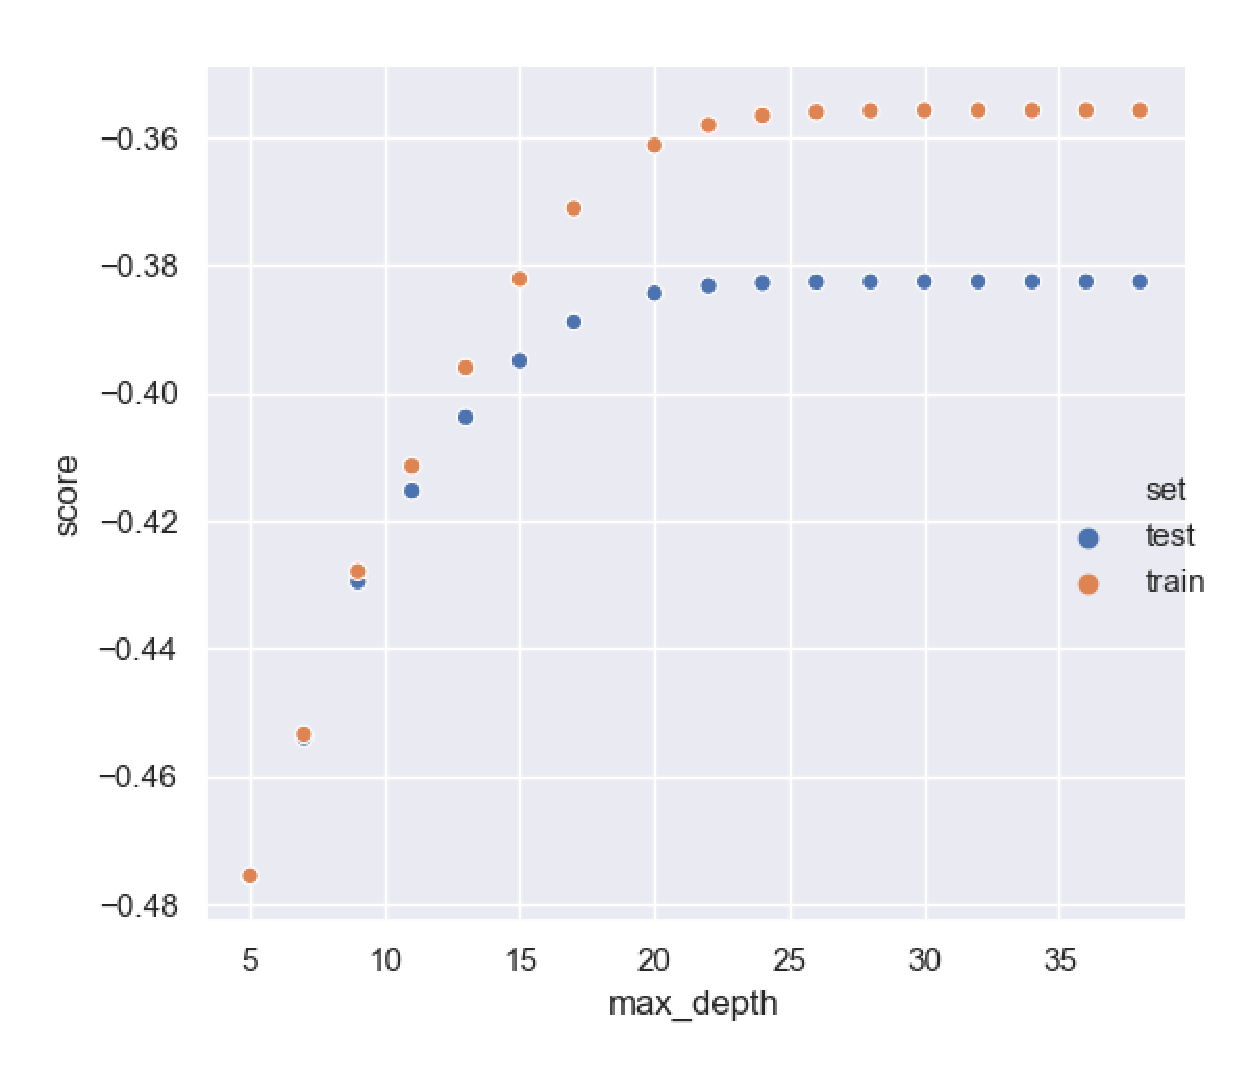
\includegraphics[width=1.0\textwidth]{figures2/max_depth_score.eps}
          \caption{Panda}
          \label{fig:source-pic}
        \end{minipage} \pause
        +
        \begin{minipage}[t]{0.3\linewidth}
          \centering
          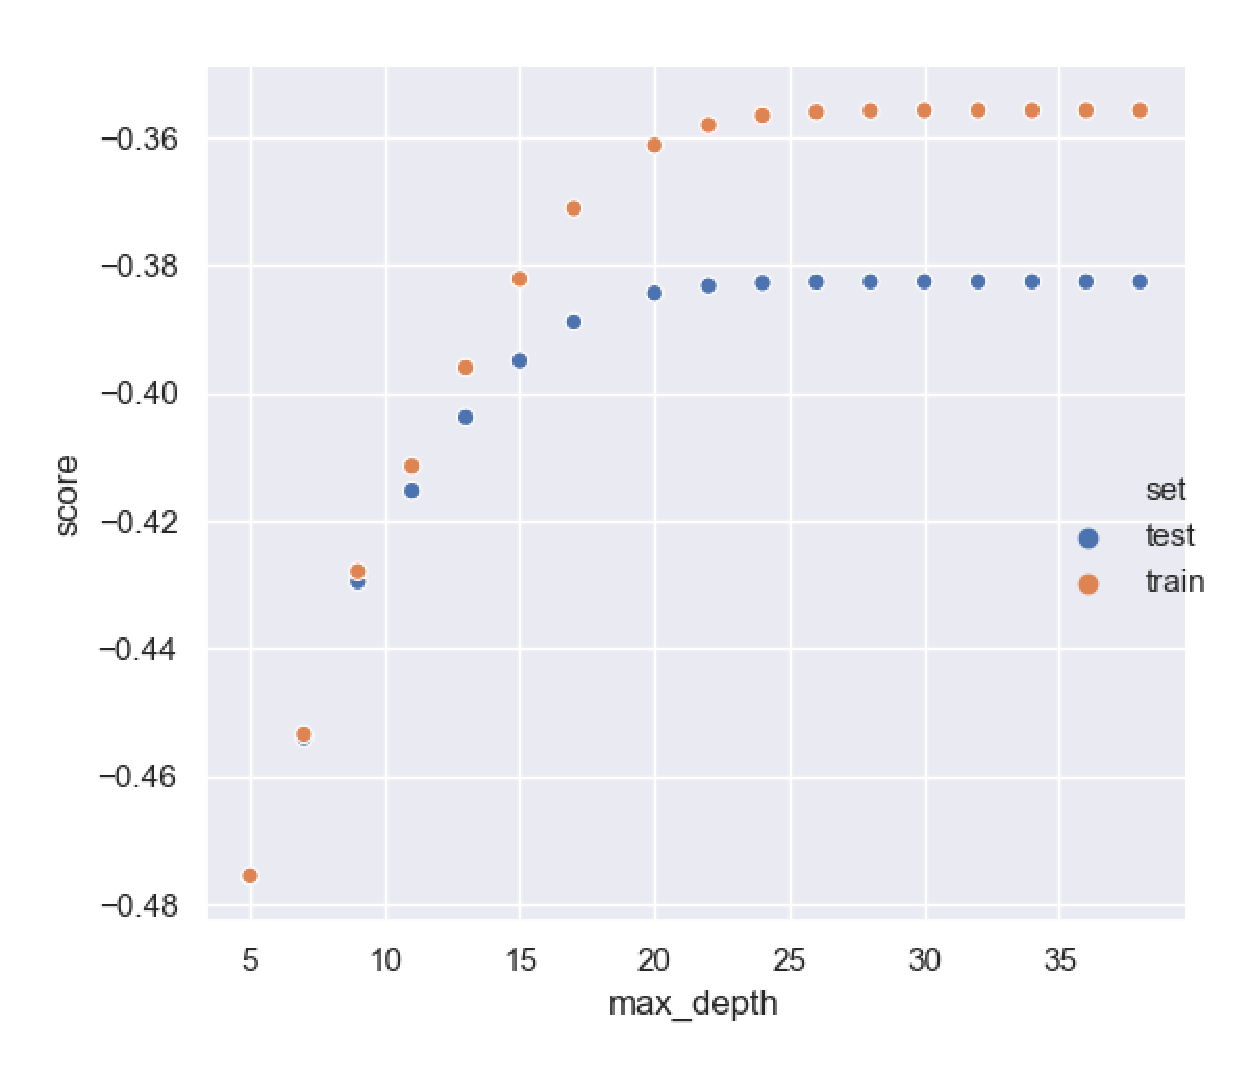
\includegraphics[width=1.0\textwidth]{figures2/max_depth_score.eps}
          \caption{Distortion}
          \label{fig:distortion}
        \end{minipage} \pause
        =
        \begin{minipage}[t]{0.3\linewidth}
          \centering
          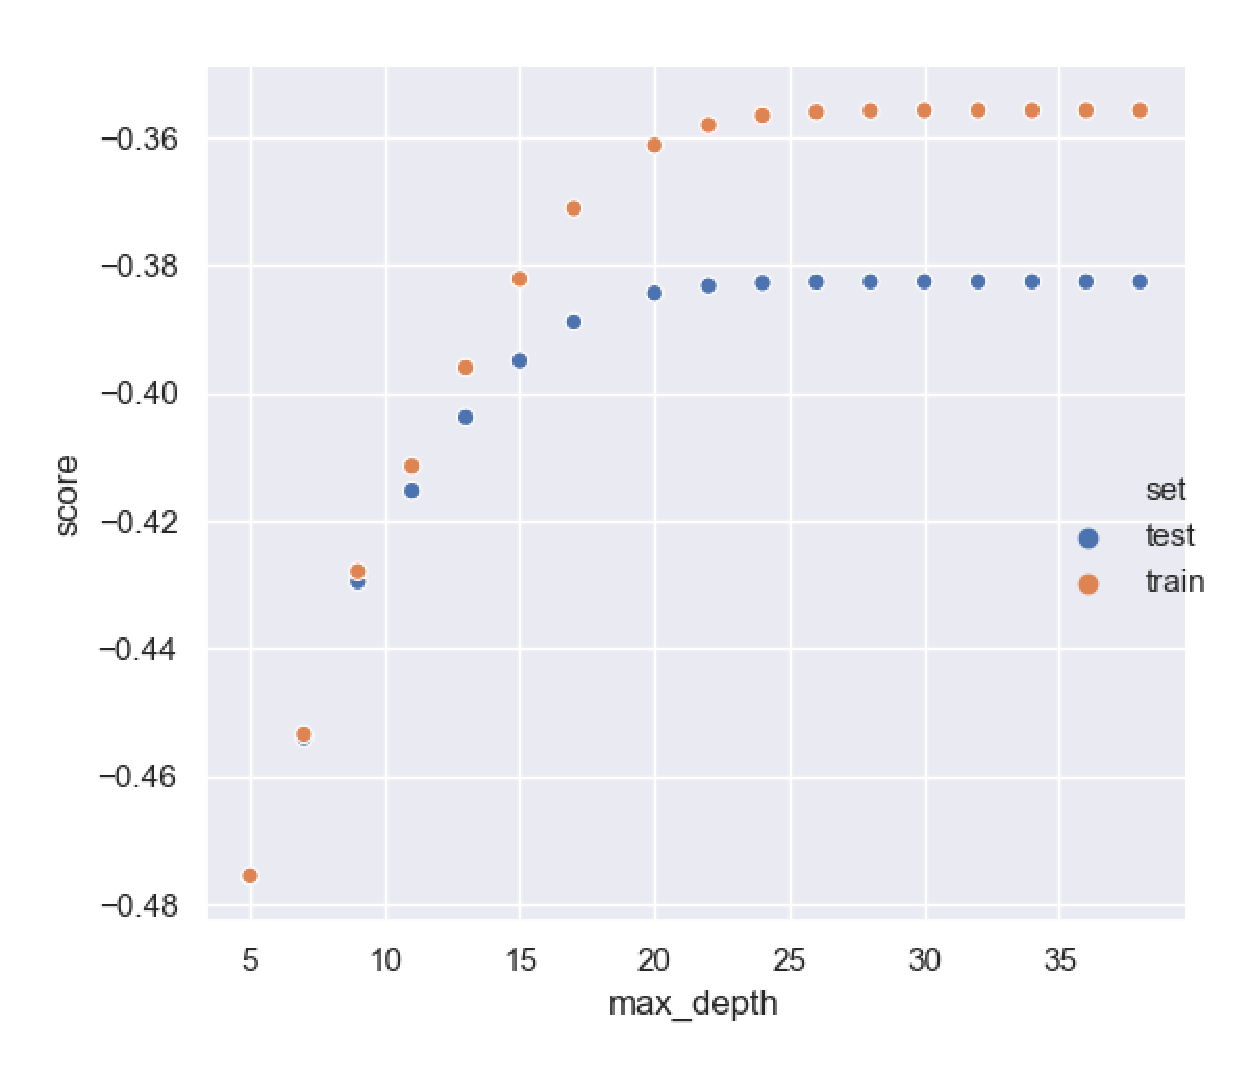
\includegraphics[width=1.0\textwidth]{figures2/max_depth_score.eps}
          \caption{Monkey}
          \label{fig:attacked-pic}
        \end{minipage}
      \end{figure}
      \item Develop an adversarial attack that causes image classifiers to predict a specific target class.
    \end{itemize}
  \end{itemize}
\end{slide}

\begin{slide}{Conditions}
  \begin{itemize}
    \item Given \pause
    \begin{figure}[h]
      \centering
      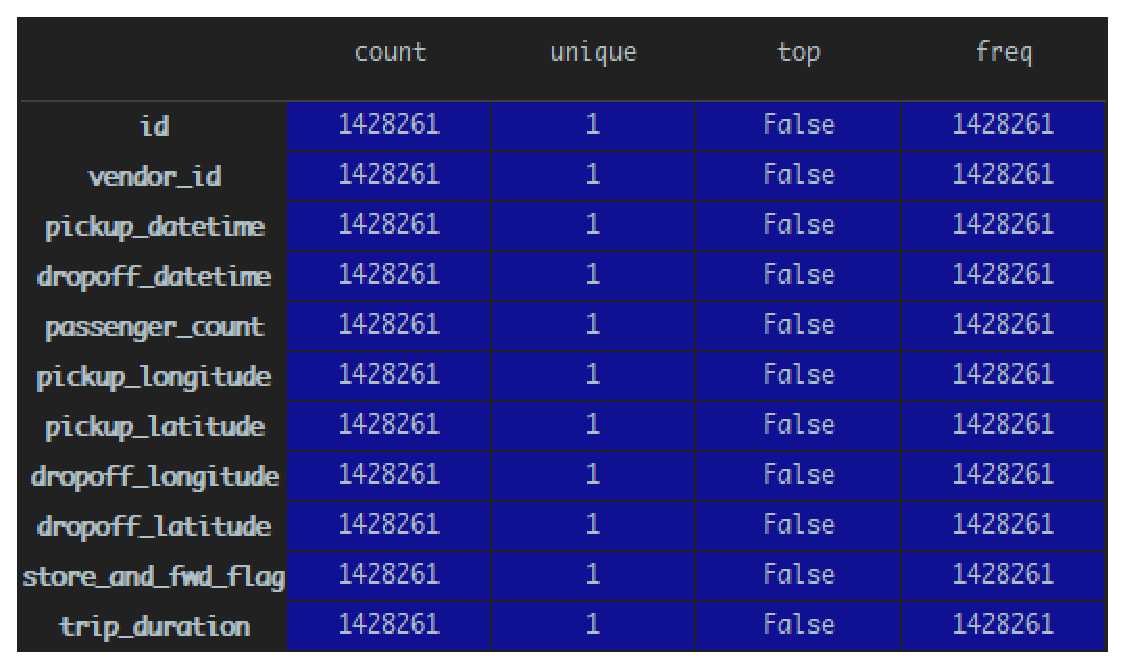
\includegraphics[width=0.4\textwidth]{figures2/train_null.eps}
      \caption{Illumination}
      \label{fig:missing-value-pic}
    \end{figure} \pause
    \begin{itemize}
      \item A set of images from ImageNet2012 which going to be attacked; \pause 
      \item The oracle at the back which was trained on dataset ImageNet2012; \pause
      \item We can never touch nor query the oracle.
    \end{itemize}
  \end{itemize}
\end{slide}

\begin{slide}{Evaluation}
  \begin{itemize}
    \item Submission \pause
    \begin{itemize}
      \item Attackers \pause
      \begin{itemize}
        \item given source images and target type; \pause
        \item return targeted attacked image; \pause
      \end{itemize}
      \item Checkpoints, dataset or anything will be used by attackers \pause
      \begin{itemize}
        \item pretrained models used by attackers; \pause
      \end{itemize}
    \end{itemize}
  \end{itemize}
  \begin{itemize}
    \item Evaluation \pause
    \begin{itemize}
      \item The evaluation metric of this competition is Root Mean Squared Logarithmic Error.
      $$
      score = \frac{num_{classified\_as\_target}}{num_{all}}
      $$ 
    \end{itemize}
  \end{itemize}
\end{slide}


\section{Researching}

\begin{slide}[toc=,bm=]{Overview of the Researching}
\tableofcontents[content=currentsection,type=0]
\end{slide}

\begin{slide}{Problems One}
  \begin{itemize}
    \item What is adversarial example, and why does it exist?
  \end{itemize}
\end{slide}

\begin{slide}{Adversarial Example}
  \begin{itemize}
    \item What?
    \begin{itemize}
      \item Adversarial examples are those examples made by adding source examples with lightly distortion, which is well-designed on purpose to fooling a classifier to make a mistake.
    \end{itemize}
    \item Features \pause
    \begin{itemize}
      \item Fools classifiers \pause
      \item Transitivity between different classifiers \pause
      \item Too small to distinguish for human eyes \pause
    \end{itemize}
  \end{itemize}
\end{slide}

\begin{slide}{Nonlinearity of model}
  \begin{itemize}
    \item Why? \pause
    \begin{itemize}
      \item Nonlinearity of model \cite{RN143} \pause
      \begin{itemize}
        \item Formula for computing volume of n-dim sphere with radius of $R$: \pause
        $$
        V_{sphere} = K * R ^ n
        $$ \pause
        \item Rate of a sphere with radius of $0.9R$ in one with radius of $R$ in n-dim space: \pause
        $$
        proportion = \frac{K*(0.9*R)^n}{K*R^n} = 0.9^n
        $$
        \pause
        \begin{figure}[h]
          \centering
          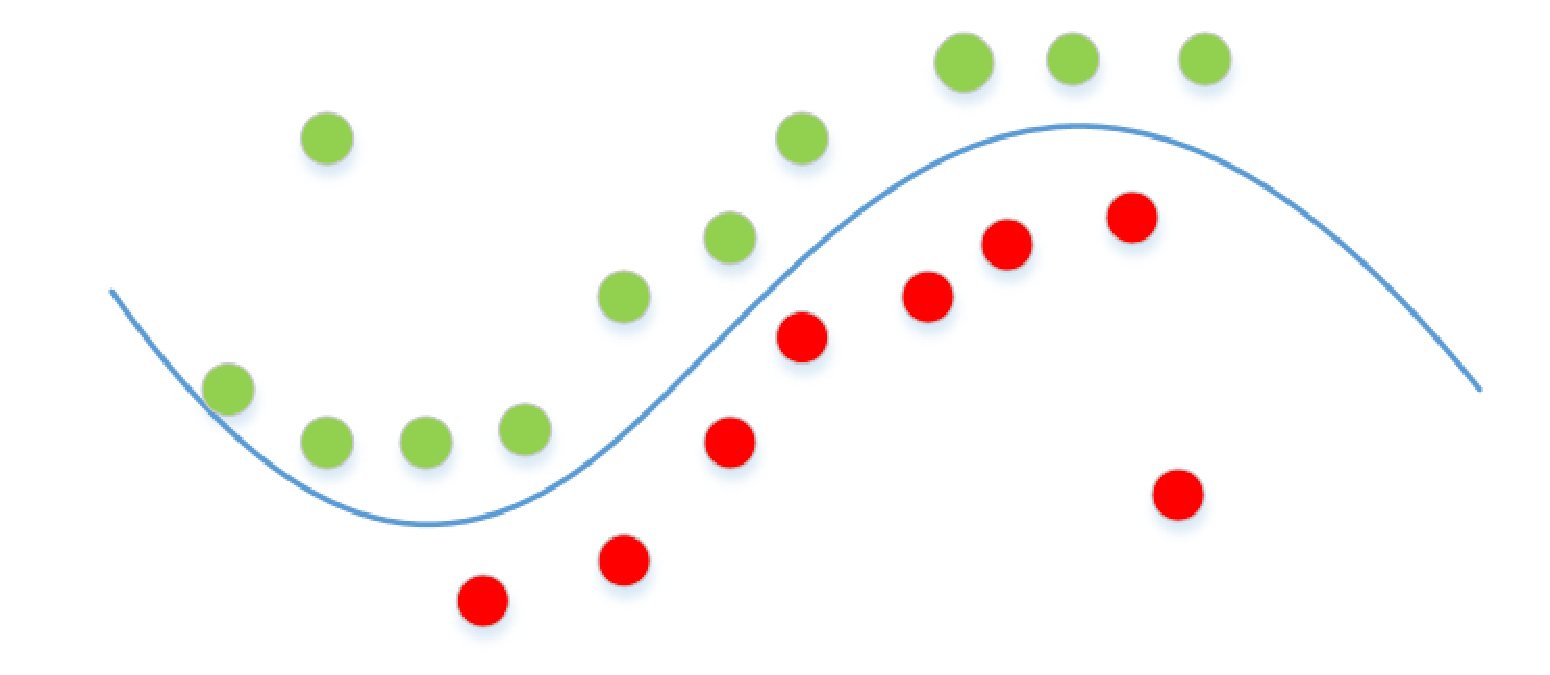
\includegraphics[width=0.5\textwidth]{figures3/density.eps}
          \caption{Illumination of vulnerability of nonlinearity model}
          \label{fig:illumination-of-nonlinearity}
        \end{figure}
      \end{itemize} 
    \end{itemize}
  \end{itemize}
\end{slide}

\begin{slide}{Linearity of model}
  \begin{itemize}
    \item Why?
    \begin{itemize}
      \item Nonlinearity of model \cite{RN143}
      \item Linearity of model \cite{RN48} \pause
      \begin{itemize}
        \item Adversarial example $\tilde{x}$ with distortion $\eta$ for source $x$ in linear model: \pause
        $$
        \omega^T \tilde{x} = \omega^T x + \omega^T \eta, 
        \left\|\eta\right\|_\infty \le \epsilon
        $$ \pause
        \item If $\epsilon $ equals to 1 which means 1 pixel, then to maxize the distortion $\omega^T\eta$: \pause
        $$
        \eta = sign(\omega)
        $$ \pause
        \item Then for average magnitude of $M$, the distortion is: \pause
        $$
        \omega^T\eta = \sum_{i=1}^{n}{\left\|\omega_i\right\|} = nM, \lim_{n\to\infty} \to \infty
        $$
      \end{itemize}
    \end{itemize}
  \end{itemize}
\end{slide}

\begin{slide}{Problems Two}
  \begin{itemize}
    \item What is adversarial example, and why does it exist?
    \item How to generate an adversarial example that fools a given classifier?
  \end{itemize}
\end{slide}

\begin{slide}{How to Attack}
  \begin{itemize}
    \item What we want to do? \pause
    \begin{figure}[h]
      \centering
      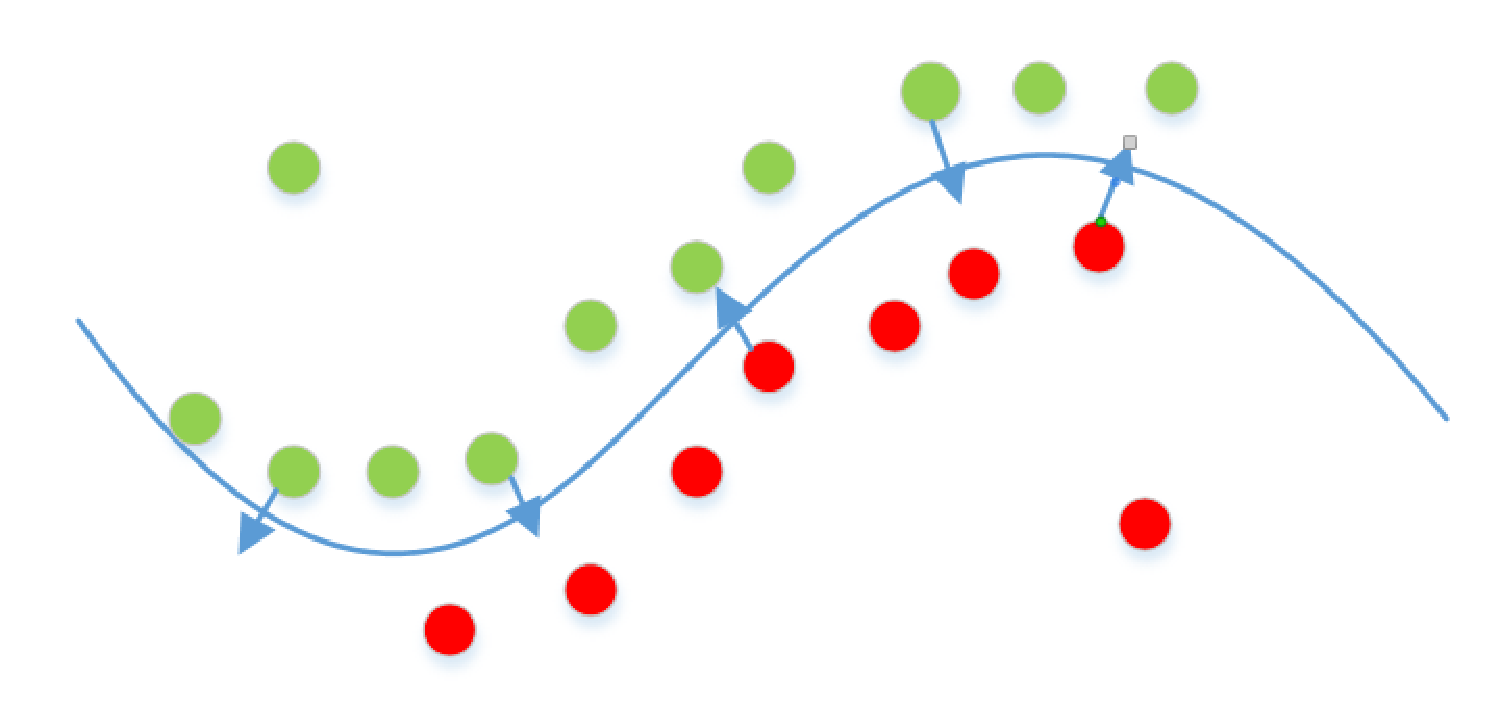
\includegraphics[width=0.5\textwidth]{figures3/wannado.eps}
      \caption{Illumination of cross the line}
      \label{fig:illumination-of-wannado}
    \end{figure} \pause
    \item How to do it? \pause
    \begin{itemize}
      \item Solve the formula:
      \begin{equation}
        \begin{split}
        &\min{\eta} \\
        &s.t. f(x+\eta) = target \pause \Leftrightarrow s.t. argmax(preds) = target
        \end{split}
      \end{equation} \pause
      
    \end{itemize}
  \end{itemize}
\end{slide}

\begin{slide}{Solve the problem}
  \begin{itemize}
    \item Formula:
    \begin{equation}
      \begin{split}
      &\min{\eta} \\
      &s.t. argmax(preds) = target
      \end{split}
    \end{equation}  \pause
    \item It is hard to solve this problem directly \pause
    \begin{itemize}
      \item Convert to unbounded problems \pause
    \end{itemize}
    \item Approximate the optimal solution \pause
    \begin{itemize}
      \item Gradient descent methods, like RMSprop, Momentum, Adam, etc.
    \end{itemize}
  \end{itemize}
\end{slide}


\section{Defenses}

\begin{slide}[toc=,bm=]{Overview of the Defenses}
\tableofcontents[content=currentsection,type=0]
\end{slide}

\begin{slide}{Adversarial training}
  \begin{itemize}
    \item Adversarial training \cite{gong2017adversarial} \pause
    \begin{figure}[h]
      \begin{minipage}[t]{0.45\linewidth}
        \centering
        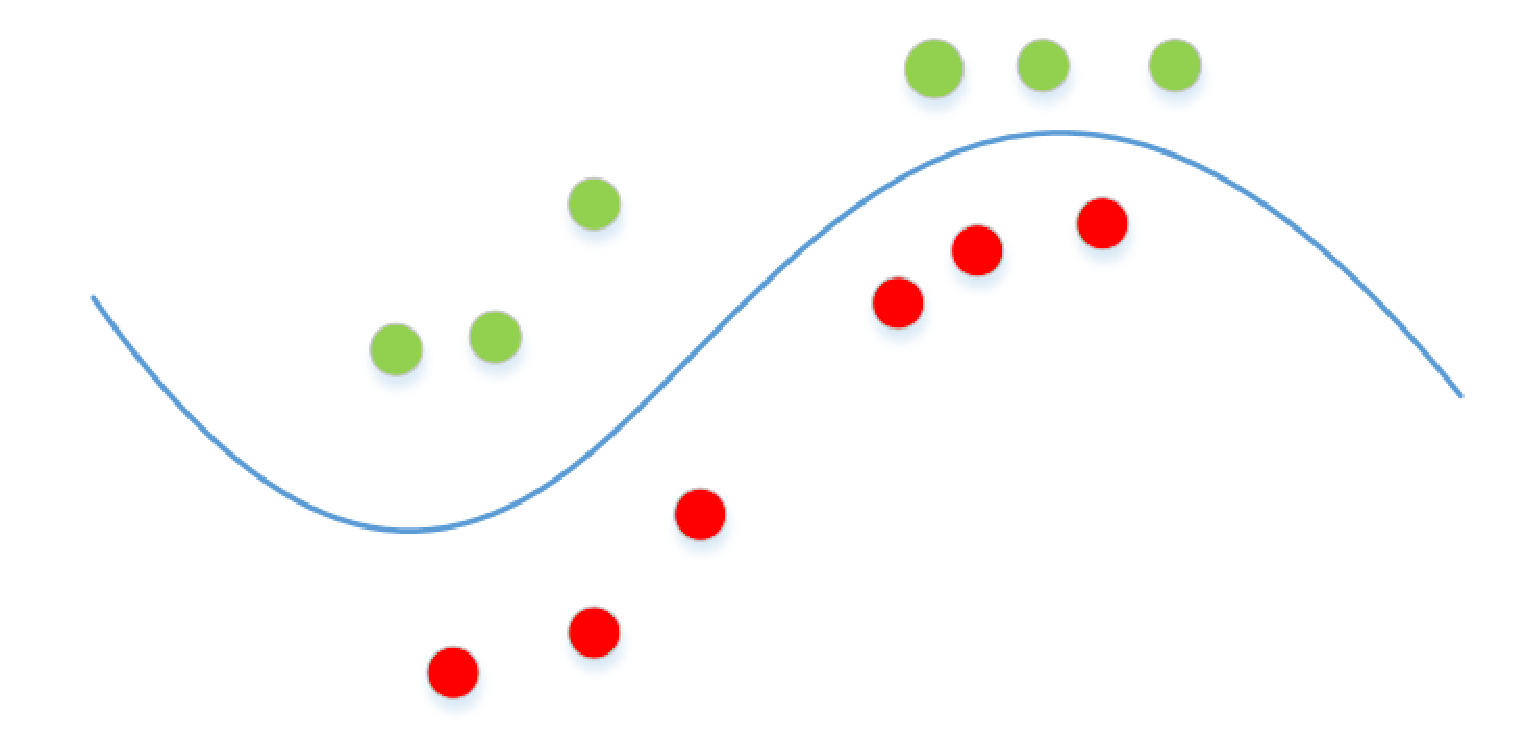
\includegraphics[width=1.0\textwidth]{figures3/beforeat.eps}
        \caption{Before Adversarial Training}
        \label{fig:before-at}
      \end{minipage} 
      \pause
      \begin{minipage}[t]{0.45\linewidth}
        \centering
        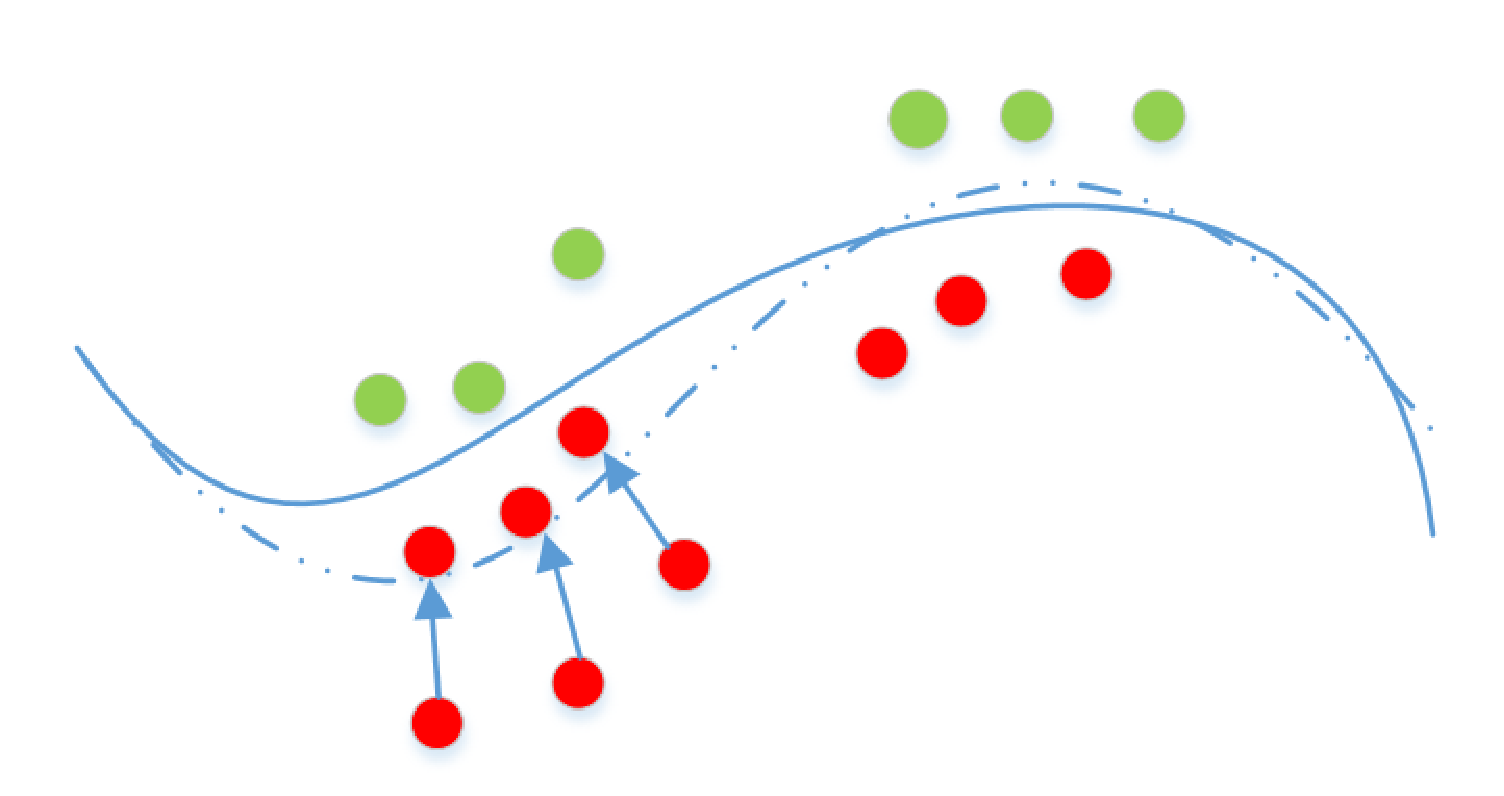
\includegraphics[width=1.0\textwidth]{figures3/afterat.eps}
        \caption{After Adversarial Training}
        \label{fig:after-at}
      \end{minipage}
    \end{figure}
  \end{itemize}
\end{slide}

\begin{slide}{Distilling}
  \begin{itemize}
    \item Distilling \cite{RN49} \pause
    \begin{figure}[h]
      \centering
      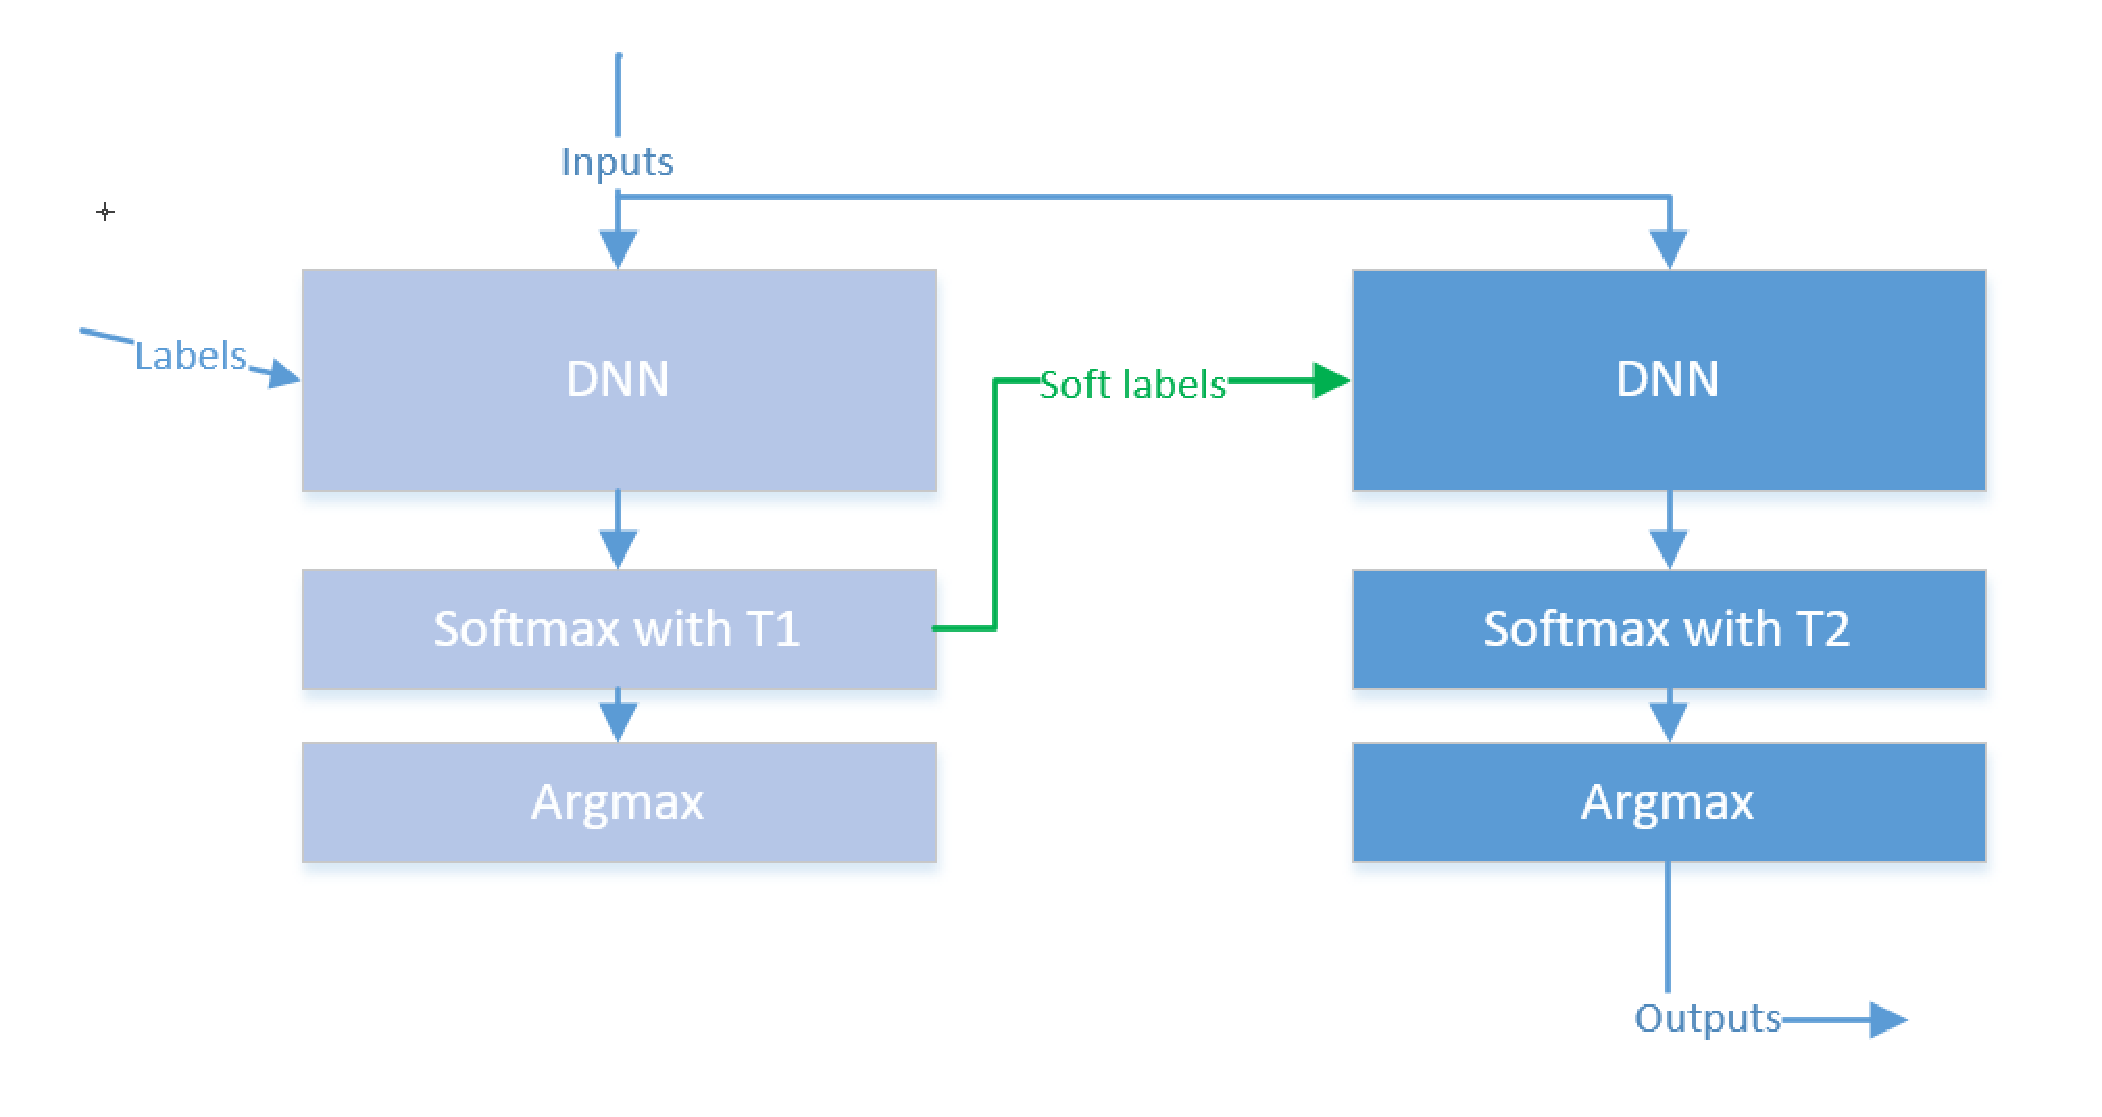
\includegraphics[width=0.7\textwidth]{figures3/distilled.eps}
      \caption{Distilled model}
      \label{fig:distilled-model}
    \end{figure}
  \end{itemize}
\end{slide}

\begin{slide}{Gradient Masking}
  \begin{itemize}
    \item Select or construct model that has small gradient \pause
    \begin{itemize}
      \item Affect the model's accuracy
      \item More hard to train 
    \end{itemize}
  \end{itemize}
\end{slide}

% \begin{slide}{Problems Four}
%   \begin{itemize}
%     \item How could I make sure the generated adversarial example also fools the oracle? \pause
%     \begin{itemize}
%       \item Adversarial examples are transmissible.
%     \end{itemize}
%   \end{itemize}
% \end{slide}


\section{Attackers}

\begin{slide}[toc=,bm=]{Overview of the Attackers}
\tableofcontents[content=currentsection,type=0]
\end{slide}

\begin{slide}{L-BFGS\cite{RN143}}
  \begin{itemize}
    \item Solve the formula:
      \begin{equation}
        \begin{split}
        &\min {\eta} \\
        &s.t. argmax(preds) = target
        \end{split}
      \end{equation} \pause
    \item Convert to an unbounded problem: \pause
    \begin{equation}
      \begin{split}
      min{c\vert\eta\vert + cross_entropy_loss_f(x+\eta, target)}
      \end{split}
    \end{equation} 
    \item Approximate the optimal $\eta^*$ by L-BFGS method
  \end{itemize}
\end{slide}

\begin{slide}{FGSM\cite{RN48}}
  \begin{itemize}
    \item Solve the formula:
      \begin{equation}
        \begin{split}
        &\min {\eta} \\
        &s.t. argmax(preds) = target
        \end{split}
      \end{equation} \pause
    \item Convert to dual problem: \pause
      \begin{equation}
        \begin{split}
        &\max {\vert f(x+\eta)-f(x) \vert} \\
        &s.t. \eta \le \epsilon
        \end{split}
      \end{equation} \pause
    \item Given the gradient $\bigtriangledown_xJ(x, y)$, we get:
      \begin{equation}
        \begin{split}
          \eta^* = sign(\bigtriangledown_xJ(x, y))
        \end{split}
      \end{equation} \pause
    \item Under the linear model, we get:
    \begin{equation}
      \begin{split}
        \eta^* = sign(\omega)
      \end{split}
    \end{equation}
  \end{itemize}
\end{slide}

\begin{slide}{FGM}
  \begin{itemize}
    \item FGM is a generalization fo FGSM
    \item Instead of just take the sign:
      \begin{equation}
        \begin{split}
          \eta^* = sign(\bigtriangledown_xJ(x, y))
        \end{split}
      \end{equation} \pause
    \item Take the gradient directly:
    \begin{equation}
      \begin{split}
        \eta^* = \bigtriangledown_xJ(x, y)
      \end{split}
    \end{equation}
  \end{itemize}
\end{slide}

\begin{slide}{I-FGM}
  \begin{itemize}
    \item Improve version of FGM \pause
    \item Instead of one-step approach:
    \begin{equation}
      \begin{split}
        \eta^* = \bigtriangledown_xJ(x, y)
      \end{split}
    \end{equation}
    \item Iteratively apply FGM:
    \begin{equation}
      \begin{split}
        \eta^* &= \eta^* + \frac{\bigtriangledown_xJ(x_{k}, y)}{\|\bigtriangledown_xJ(x_{k}, y)\|} \\
        x_{k+1} &= x_{k} + \alpha \dot \eta^*
      \end{split}
    \end{equation}
  \end{itemize}
\end{slide}

\begin{slide}{IM-FGM\cite{RN144}}
  \begin{itemize}
    \item Based on I-FGM: \pause
    \begin{equation}
      \begin{split}
        \eta^* &= \eta^* + \frac{\bigtriangledown_xJ(x_{k}, y)}{\|\bigtriangledown_xJ(x_{k}, y)\|} \\
        x_{k+1} &= x_{k} + \alpha \dot \eta^*
      \end{split}
    \end{equation} \pause
    \item Improve with momentum: \pause
    \begin{equation}
      \begin{split}
        \eta^* &= \eta^* + \alpha \frac{g_{k+1}}{\|g_{k+1}\|} \\
        x_{k+1} &= x_{k} + \alpha \dot \eta^* \\
        g_{k+1} &= \mu \dot g_k + \frac{\bigtriangledown_xJ(x_{k}, y)}{\|\bigtriangledown_xJ(x_{k}, y)\|}
      \end{split}
    \end{equation}
  \end{itemize}
\end{slide}

\begin{slide}{C\&W\cite{RN139}}
  \begin{itemize}
    \item Solve the formula:
      \begin{equation}
        \begin{split}
        &\min {\eta} \\
        &s.t. argmax(preds) = target
        \end{split}
      \end{equation} \pause
    \item Convert to unbounded problem \pause
    \begin{equation}
      \begin{split}
      \min {\alpha\|\eta\|_2 + max\{Z(x)_{i\neq target}\}-Z(x)_{target}}
      \end{split}
    \end{equation} \pause
    \begin{figure}[h]
      \begin{minipage}[t]{0.25\linewidth}
        \centering
        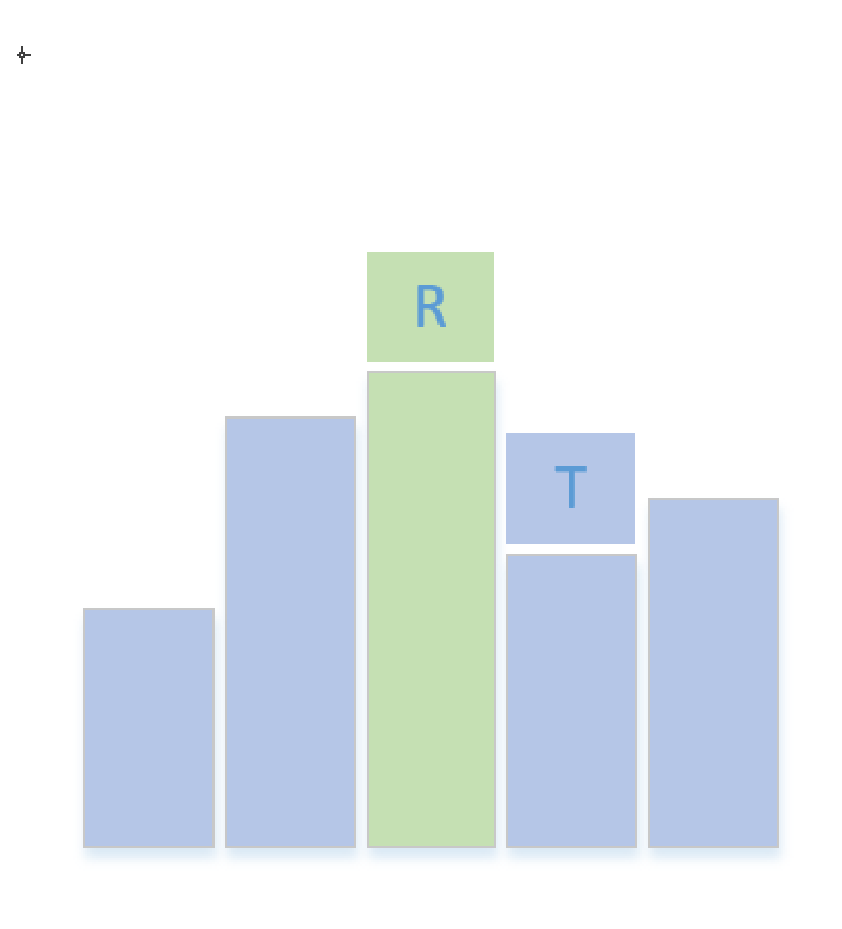
\includegraphics[width=1.0\textwidth]{figures3/feasible.eps}
        \caption{Feasible solution}
        \label{fig:feasible-solution}
      \end{minipage} 
      \pause
      \begin{minipage}[t]{0.25\linewidth}
        \centering
        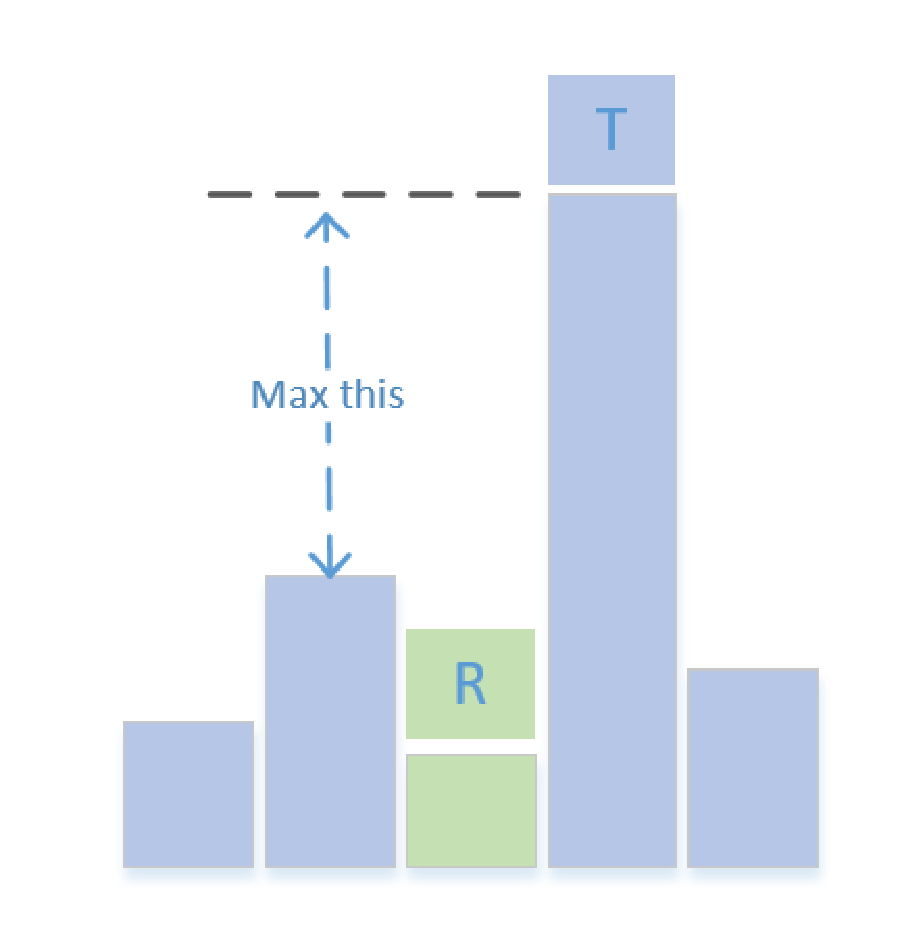
\includegraphics[width=1.0\textwidth]{figures3/optimal.eps}
        \caption{Optimal}
        \label{fig:optimal-solution}
      \end{minipage}
    \end{figure}
  \end{itemize}
\end{slide}


\begin{slide}{EAD\cite{RN139}}
  \begin{itemize}
    \item Based on C\&W: \pause
    \begin{equation}
      \begin{split}
      \min {\alpha\|\eta\|_2 + max\{Z(x)_{i\neq target}\}-Z(x)_{target}}
      \end{split}
    \end{equation} \pause
    \item Add one more limit condition:
    \begin{equation}
      \begin{split}
      \min {\alpha\|\eta\|_1 + \beta\|\eta\|_2 + max\{Z(x)_{i\neq target}\}-Z(x)_{target}}
      \end{split}
    \end{equation} \pause
    \item Solve with ISTA:
    \begin{itemize}
      \item Given that:
      \begin{equation}
        \begin{split}
          g(x) &= \beta\|\eta\|_2 + max\{Z(x)_{i\neq target}\}-Z(x)_{target}
        \end{split}
      \end{equation}
      \item Compute iteratively:
      \begin{equation}
        \begin{split}
          x_{k+1} &= S_{\beta}(x_{k} + \alpha \bigtriangledown_g(x_k))
        \end{split}
      \end{equation}
    \end{itemize}
  \end{itemize}
\end{slide}

\section{Experiments}

\begin{slide}[toc=,bm=]{Overview of the Researching}
\tableofcontents[content=currentsection,type=0]
\end{slide}

\begin{slide}{Plan}
  \begin{itemize}
    \item Build a distilled model as the oracle enabled defense \pause
    \item Create attackers to attack the local oracle \pause
    \item Test and evaluate them on Mnist dataset first \pause
    \item Select and fine tune attackers \pause
    \item Test and evaluate on the given dataset \pause
  \end{itemize}
\end{slide}


% \begin{slide}{Rank of Competition}
%   \begin{itemize}
%     \item Score: 0.41895
%     \item Rank: 545/1207
%   \end{itemize}
%   \begin{figure}[h]
%     \centering
%     
\includegraphics[width=0.8\textwidth]{figures2/score.eps}
%     \caption{Result of the best submission}
%     \label{fig:result-of-best-submission}
%   \end{figure} 
% \end{slide}


\section{Summary}

\begin{slide}{Thanks}
  \begin{itemize}
    \item Thanks for listening~
  \end{itemize}
\end{slide}
  
% \begin{slide}{References (1)}
% \bibliographystyle{plain}
% \nobibliography{YourBib}
% \bibentry{someone1}
% \bibentry{someone2}
% \end{slide}

% \begin{slide}{References (2)}
% \bibentry{someone3}
% \end{slide}

% \begin{slide}{Slide}
% \cite{someone}
% \end{slide}
% 
\begin{slide}{References}
  \bibliographystyle{plain}
  \bibliography{mybib}
\end{slide}

\end{document}

\endinput
